% filepath: /Users/lorenzo.speri/Library/CloudStorage/OneDrive-ESA/Documents/GitHub/ResponseRequirements/results_report.tex
\documentclass[a4paper,12pt]{article}
\usepackage{graphicx}
\usepackage{caption}
\usepackage{subcaption}
\usepackage{amsmath}
\usepackage{hyperref}
\usepackage{geometry}
\geometry{margin=1in}

\title{Results Report}
\author{}
\date{\today}

\begin{document}

\maketitle

% \tableofcontents
% \newpage

\section{Introduction}
This document presents the results of the impact of uncertainty on the LISA spacecraft positions on the TDI outputs of a gravitational wave signal, here assumes to be a galactic binary. The analysis is based on the LISA TDI framework and includes the calculation of mismatch for the channels (A, E, T). 
The analysis is performed for different values of the frequency $f$ and averaged over different inclination, polarization angles and sky location parameters. The spacecrafts are in a heliocentric orbit for one year. The spacecrafts are located at the vertices of an equilateral triangle with a side length of 2.5 million km as shown in Figure~\ref{fig:lisa_orbit}. 
 
\begin{figure}
    \centering
    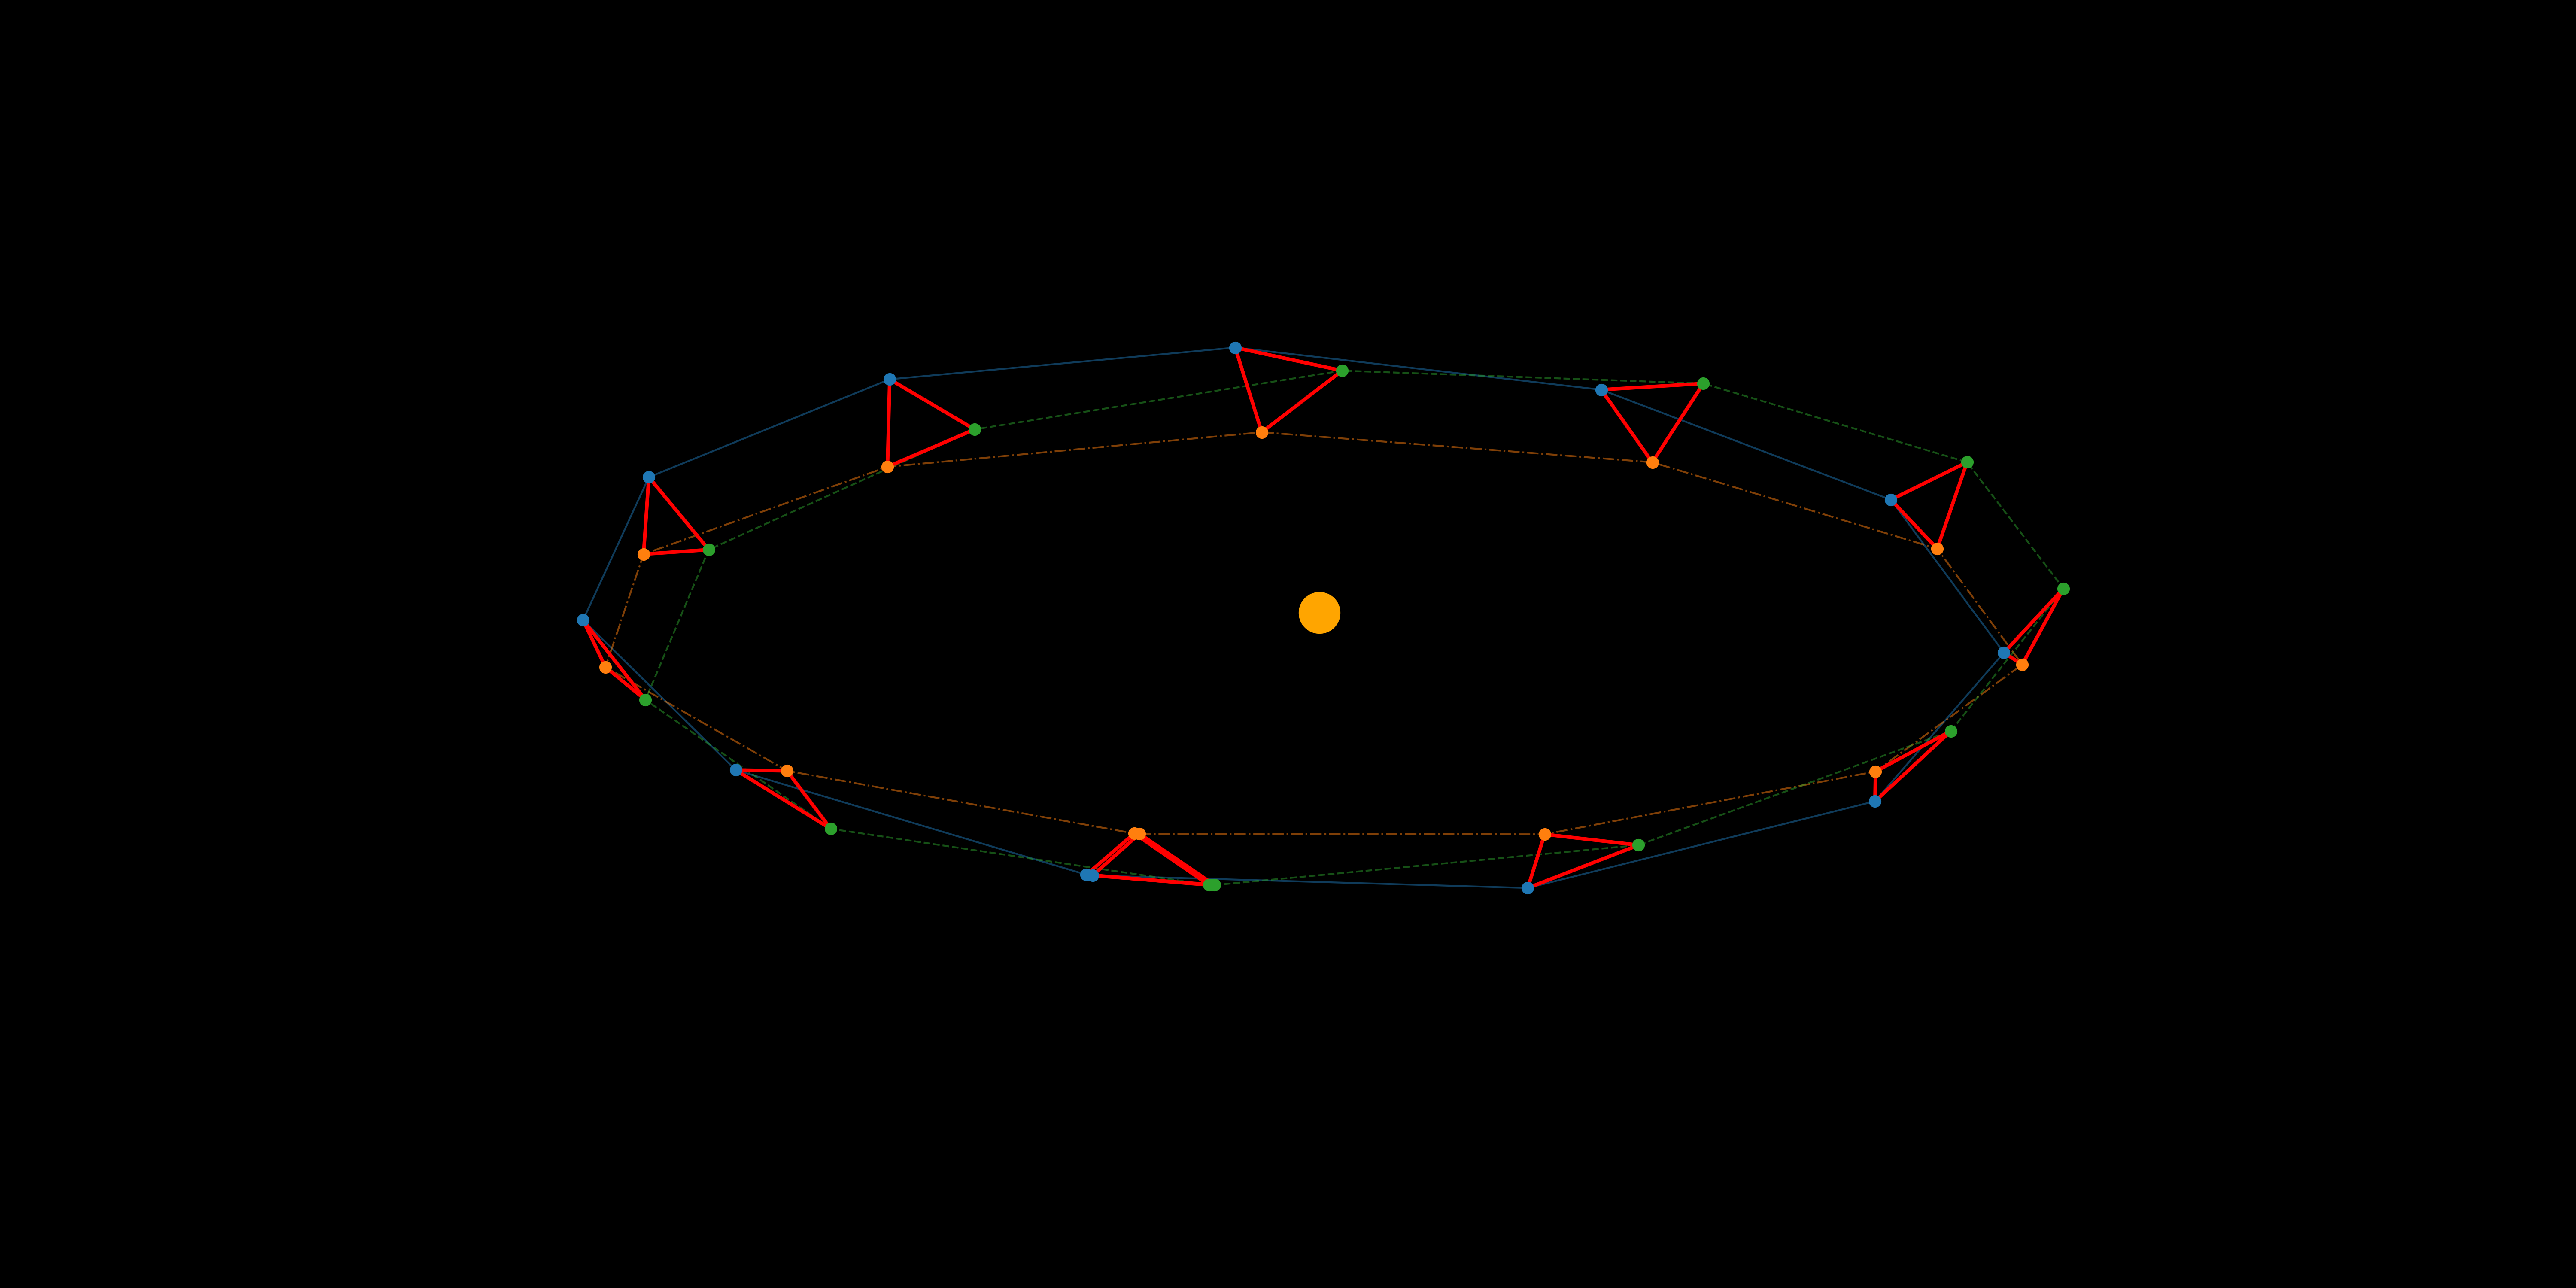
\includegraphics[width=0.9\textwidth]{figures/3d_orbit_around_sun.png}
    \caption{LISA orbit around the Sun for one month.}
    \label{fig:lisa_orbit}
\end{figure}

We vary the orbits of the LISA spacecrafts according the worst values of \href{https://doi.org/10.1007/s40295-021-00263-2}{Trajectory Design for the ESA LISA Mission} which are of order $10^3$ kms in the LISA local frame. This leads to variation in the spacecraft positions as shown in Figure\ref{fig:sc_deviation}.

\begin{figure}
    \centering
    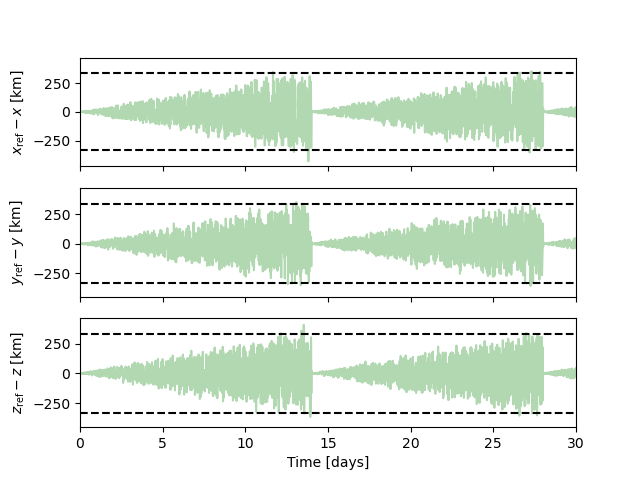
\includegraphics[width=0.9\textwidth]{figures/orbits_deviation.png}
    \caption{LISA spacecraft 1 position deviations in the SSB frame for 1-sigma values.}
    \label{fig:sc_deviation}
\end{figure}

\begin{figure}
    \centering
    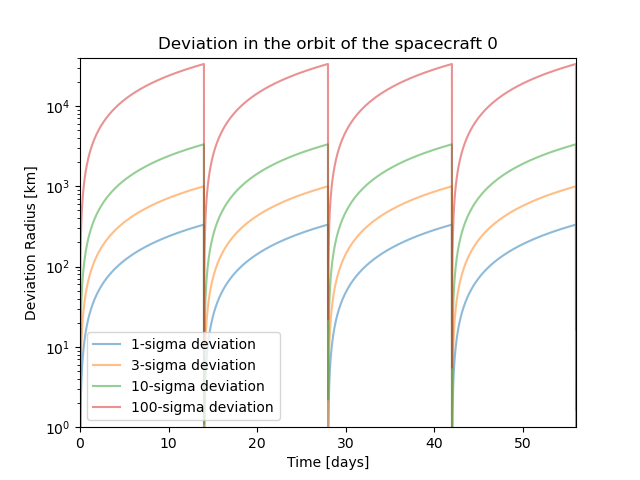
\includegraphics[width=0.9\textwidth]{figures/radius_deviation.png}
    \caption{Radius of the deviation for LISA spacecraft 1 for different sigma values.}
    \label{fig:sc_radius_deviation}
\end{figure}


\section{Mismatch Plots}
The following figures show the mismatch 95\% upper bounds for different $\sigma$ values and channels (A, E, T).

\begin{figure}[h!]
    \centering
    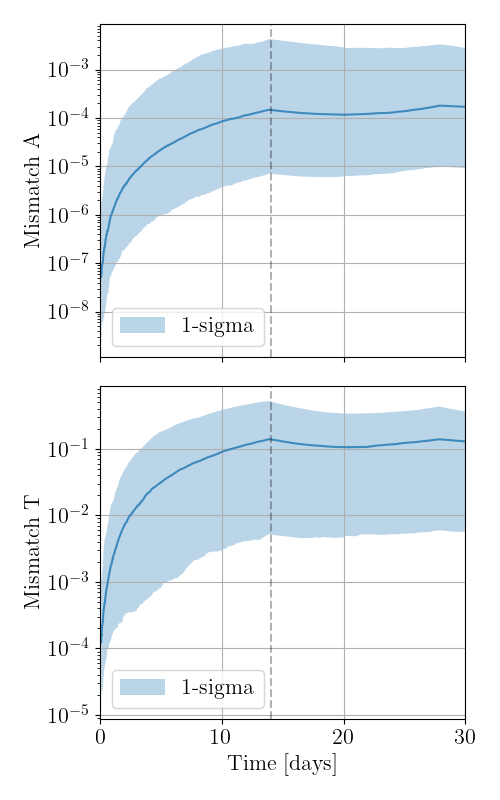
\includegraphics[width=\textwidth]{figures/mismatch_upper95_tdi_deviation_A1e-22_f0.0001_fdot1.5e-17.png}
    \caption{Mismatch 95\% upper bound for all channels and $\sigma$ values.}
    \label{fig:mismatch_upper95_1e-4}
\end{figure}


\section{Conclusion}
The results demonstrate the behavior of mismatch and RMS for different $\sigma$ values and channels. The sky location scatter plots provide additional insights into the relationship between mismatch and sky location parameters.

\end{document}